\documentclass{article}

\usepackage{amsmath}
\usepackage{amsthm}
\usepackage{amssymb}
\usepackage{graphicx}

\usepackage{hyperref}
\usepackage{fullpage}

\newcommand{\smallest}{\operatornamewithlimits{smallest}}

\DeclareMathOperator*{\argmin}{arg\!min}
\DeclareMathOperator*{\var}{var}

\begin{document}

\title{Coarse-to-fine Gaussian Process Regression}
\author{Yusuf Erol and Dave Moore}
\date{March 13, 2012}
\maketitle

\section{Introduction}

Gaussian processes are a powerful tool for nonlinear regression. Gaussian process regression (GPR) is nonparametric, enabling it to represent increasingly complex functions as the amount of training data increases, and unlike most other kernel-based methods, it is also inherently probabilistic: it provide not just a single prediction of the function value at a test point, but a full probability distribution. This principled approach to uncertainty makes GPs ideal for use as part of larger Bayesian models, as well as enabling a wide range of additional applications including active learning, optimal sensor placement, and global function optimization \cite{guestrin2005near}\cite{osborne2009gaussian}. 

However, all of this power comes at a cost. Training a GP model requires $O(n^3)$ time and $O(n^2)$ space in the number of training examples, while making a single prediction requires $O(n)$ time (including $n$ evaluations of the kernel function). For this reason, na\"{\i}ve GP regression is infeasible on large datasets; for example, training a model with $n = 100000$ requires on the order of a quadrillion operations. Clearly, significant improvements are necessary in order to scale GP regression (and kernel regression in general) to modern ``big data'' problems with millions or billions of training examples. In this report, we briefly review Gaussian process regression, then describe several previously proposed approaches for efficiently learning approximate models, and finally discuss potential directions for improving on these approaches. 

\section{Gaussian Process Regression}
In the regression task, our goal is to learn some unknown function $f({\mathbf x})$. We are given as training data a set of $n$ points $\mathbf{X} = \{\mathbf{x}_1, \ldots, \mathbf{x}_n\}$, along with a vector $\mathbf{y} = [y_1, \ldots, y_n]$ containing observations of the function evaluated at each point. We assume the observations are noisy; that is, $y_i = f(\mathbf{x_i}) + \epsilon_i$ where $\epsilon_i \sim N(0, \sigma^2)$. 

The premise of Gaussian process regression is that, for any set of points $\mathbf{x}_1, \ldots, \mathbf{x}_n$, the joint distribution of the function values $[f(\mathbf{x}_1), \ldots, f(\mathbf{x_n})]$ is multivariate Gaussian. The mean of the Gaussian is typically taken to be zero (though this is not necessary), and the covariances are specified by a positive semidefinite kernel function $k(\mathbf{x}, \mathbf{x'})$. The specific choice of kernel determines the inductive bias of the regressor, and is the major modeling decision to be made when applying GP regression. One common choice is the {\em squared-exponential} kernel\begin{equation}[k(\mathbf{x}, \mathbf{x'}) = \exp\left (- \frac{ \|\mathbf{x} - \mathbf{x'}\|^2 }{2w} \right)\end{equation}
which decays with the distance between $\mathbf{x}$ and $\mathbf{x'}$ at a rate given by the length scale parameter $w$. 

Given a kernel and a training set, we can define the kernel matrix $\mathbf{K}$ as the $n \times n$ symmetric matrix given by $K_{ij} = k(\mathbf{x}_i, \mathbf{x_j})$. This is the covariance matrix of the function values at the training points; we extend this to $\mathbf{M} = (\mathbf{K} + \sigma^2\mathbf{I})$ to account for the additional variance introduced by the noisy observations. Then a standard derivation \cite{rasmussen06} shows that the conditional distribution $p(\mathbf{x} | \mathbf{x_1}, \ldots, \mathbf{x_n}, \mathbf{y})$ of the function value at a test point, given the training data, is Gaussian with mean and variance
\begin{align}
\mathbb{E}(f(\mathbf{x}) | \mathbf{X}, \mathbf{y}) &= \mathbf{k}^T \mathbf{M}^{-1} \mathbf{y}\\
\var(f(\mathbf{x}) | \mathbf{X}, \mathbf{y}) &= k(\mathbf{x}, \mathbf{x}) - \mathbf{k}^T \mathbf{M}^{-1} \mathbf{k}.
\end{align}
where $\mathbf{k}$ is the vector of kernel evaluations between the test point and the training point, that is $\mathbf{k}_i = k(\mathbf{x},\mathbf{x}_i)$. 

Let us consider the complexity involved in learning and prediction using these equations. The expectation at a query point consists of a dot product between two $n$-element vectors, $\mathbf{k}$ and $\mathbf{M}^{-1} \mathbf{y}$. Note that the latter vector is independent of the query point and can be precomputed during training, so the marginal cost of predicting a single new point is $O(n)$. However, training requires significantly longer: $O(n^3)$ time to compute $\mathbf{M}^{-1}$ using standard methods (e.g. Cholesky decomposition). Note that if we want to be able to predict variances we must store $\mathbf{M}^{-1}$ explicitly using $O(n^2)$ space (since $\mathbf{M}^{-1}$ will be dense in general even if $\mathbf{M}$ is sparse), whereas if we only require expectations we can precompute the vector $\mathbf{M}^{-1}\mathbf{y}$ and store it using $O(n)$ space (although $O(n^2)$ space is still required for the computation).

\section{Related Work}
As has been discussed in the earlier sections, the training requires the inversion of the Gram matrix $\mathbf{K}+\sigma^2\mathbf{I}$ which is an $N\times N$ matrix. Naive approaches for this inversion requires $O(N^3)$ operations. In the case of practical applications, N can be on the order of $10^6$ to $10^9$ and even computing and storing the Gram matrix can be prohibitive. Moreover, for big $N$, the Gram matrix has to be stored in slow memory and transferring the data from slow memory to fast memory will dominate the cost of arithmetic operations \cite{RandomizedMatrixDecompose}.  Various researchers have proposed computationally efficient techniques in order to reduce these various costs. Low rank and sparse approximations and randomized algorithms aim to reduce the cost of the matrix inversion from $O(N^3)$ to more feasible levels. There are various approaches utilizing fast matrix-vector multiplication techniques in order to reduce the costs further during training and prediction stages. Space-partitioning trees like KD-trees and cover trees have been applied as an alternative to the low rank and sparse approximations. Moreover, in order to cope with the transfer from slow memory some algorithms have been proposed that just passes over the Gram matrix once.
\subsection{Low-Rank Approximations}
The training stage requires computing the term $(\mathbf{K}+\sigma^2\mathbf{I})^{-1}\mathbf{y}$. The inversion of the Gram matrix $\mathbf{K}+\sigma^2\mathbf{I}$ or equivalently solving the linear system $(\mathbf{K}+\sigma^2\mathbf{I})\mathbf{v}=\mathbf{y}$ requires $O(N^3)$ operations. If the kernel is known to be rank q (where $q<<N$), exploiting the low-rank structure will be beneficial computationally. Even in the case of a full rank matrix, the spectrum of the eigenvalues may decay fast and this means that one can get an accurate matrix approximation in the subspace of eigenvectors with bigger eigenvalues. 

The reduced-rank approximations scheme goes as follows: A matrix $\mathbf{Q}$ is first to be found such that $\mathbf{K} \approx \mathbf{Q}\mathbf{Q}^T$ . Then the inverse Gram matrix using the matrix inversion lemma can be written as:
\begin{eqnarray}
(\mathbf{K}+\sigma^2\mathbf{I})^{-1}&=&(\mathbf{Q}\mathbf{Q}^T+\sigma^2\mathbf{I})^{-1} \nonumber \\
&=&\sigma^{-2}\mathbf{I}-\sigma^{-2}\mathbf{Q}(\sigma^2\mathbf{I}+\mathbf{Q}^T\mathbf{Q})^{-1}\mathbf{Q}^T
\end{eqnarray}
Important thing to note in this case is that one needs to invert a $q \times q$ matrix which requires $O(q^3)$ only. Therefore, whole cost of the operation in this case is finding an approximating $\mathbf{Q}$ matrix.

Reduced-rank approximations are accurate for most of the practical applications due to eigenvalue spectrum. The kernel matrix $\mathbf{K}$ is a positive-semidefinite symmetric matrix, hence its eigenvalues are real and positive. Moreover, the spectral theorem states that $\mathbf{K}=\mathbf{U\Lambda U}^T$, where $\mathbf{U}$ is a unitary matrix (i.e. $\mathbf{U}\mathbf{U}^T=\mathbf{U}^T\mathbf{U}=\mathbf{I}$) and $\mathbf{\Lambda}$ is a diagonal matrix, with eigenvalues on the diagonal. The prediction at the training points is given as :
\begin{eqnarray}
\bar{f}&=&\mathbf{K}(\mathbf{K}+\sigma^2\mathbf{I})^{-1}\mathbf{y} \nonumber \\
\bar{f}&=&\mathbf{U\Lambda U}^T(\mathbf{U\Lambda U}^T+\sigma^2\mathbf{I})^{-1}\mathbf{y} \nonumber \\
\bar{f}&=& \mathbf{U\Lambda U}^T\mathbf{U}^{-T}(\mathbf{\Lambda}+\sigma^2\mathbf{I})^{-1}\mathbf{U}^{-1}\mathbf{y} \nonumber \\
\bar{f}&=& \mathbf{U\Lambda}(\mathbf{\Lambda}+\sigma^2\mathbf{I})^{-1}\mathbf{U}^{-1}\mathbf{y} 
\end{eqnarray}
Furthermore, since the eigenvectors $\left\{\mathbf{u}_i\right\}_{i=1}^N$ form a basis for the $N$ dimensional vector space, one can easily represent any vector as a linear sum of the eigenvectors. Let's assume that $\mathbf{y}=\mathbf{U}\mathbf{\gamma}$. Then,
\begin{eqnarray}
\bar{f}&=& \mathbf{U\Lambda U}^T\mathbf{U}^{-T}(\mathbf{\Lambda}+\sigma^2\mathbf{I})^{-1}\mathbf{y}  \nonumber \\
\bar{f}&=&\sum_{i=1}^n\frac{\gamma_i\lambda_i}{\lambda_i+\sigma_n^2}\mathbf{u}_i
\end{eqnarray}
Therefore, if $\frac{\lambda_i}{\lambda_i+\sigma^2}<<1$, then the component along $\mathbf{u}_i$ is negligible. In this case, the reduced-rank approximation of rank $q$ will be:
\begin{equation}
K\approx \sum_{i=1}^q \lambda_i \mathbf{u}_i \mathbf{u}_i^T; \> where \> \lambda_1\geq \lambda_2 \geq \dots \lambda_n
\end{equation}
The issue with this approach is that it requires knowing the spectrum of the eigenvalues which indeed costs $O(N^3)$.  Several approaches have been proposed in order to have a cheaper eigenvalue decomposition \cite{rasmussen06}. 

One particular approach is Nystrom method which approximates the eigenvectors of the kernel matrix by choosing a subset of data. In order to choose subsets of data several greedy algorithms have been proposed \cite{rasmussen06} \cite{smolaGreedy}. A randomized matrix approximation approach is given in \cite{RandomizedMatrixDecompose} which is also a \textit{single pass} algorithm. 

Assuming that the subspace of interest (the eigenvectors with substantial eigenvalues) is obtained, one can try to solve the linear system in the subspace of interest using an iterative technique like Conjugate Directions. Intuitively, this is equivalent to projecting the true solution vector to the subspace of interest.
\begin{figure}[b!] \label{fig:subspace}
  \caption{Solution in the Subspace of Interest}
  \centering
    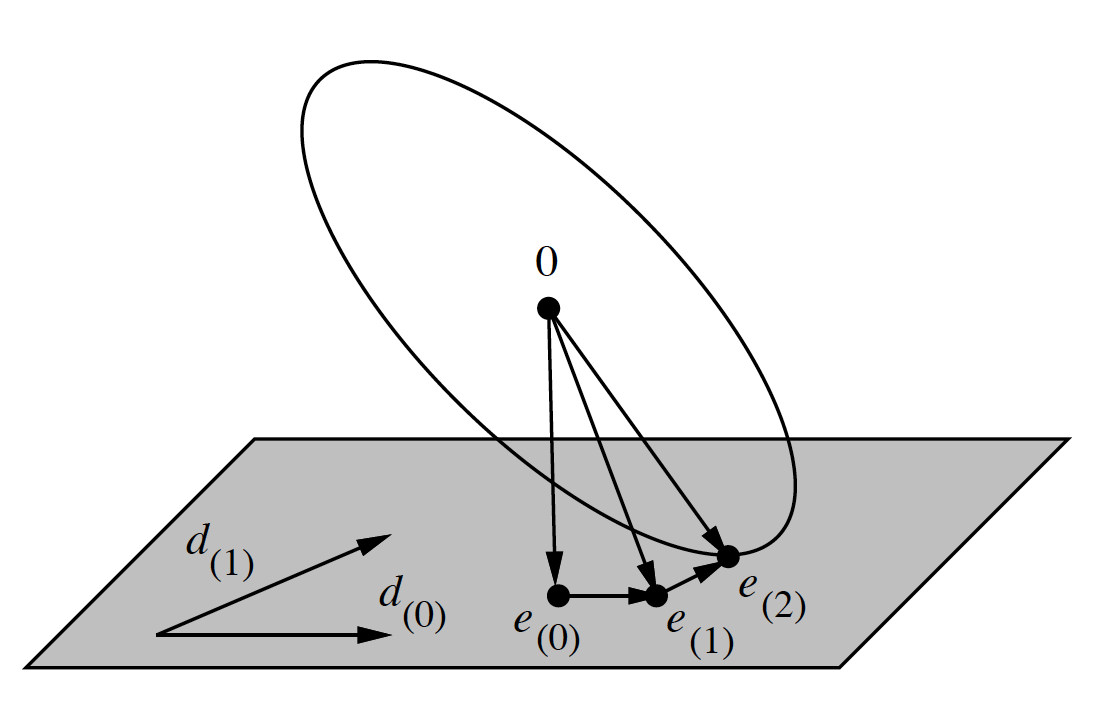
\includegraphics[width=0.7\textwidth]{subspace}
\end{figure}
A pictorial description of solving the linear system in a subspace is given in figure \ref{fig:subspace}
\subsection{Random Features}
Idea of random features is approximating the kernel using a randomized feature map $\mathbf{z}$ and expressing the problem as a linear machine problem \cite{randomfeatures}. 
\begin{equation}
k(\mathbf{x},\mathbf{x'})=<\phi(\mathbf{x})\phi(\mathbf{x'})>\approx \mathbf{z}(\mathbf{x})^T\mathbf{z}(\mathbf{x'}); \>where\> \mathbf{x} \in \mathbb{R}^d
\end{equation}
For the frequently used stationary kernels, one can utilize the Random Fourier Features. For a stationary kernel $k(\mathbf{x},\mathbf{x'})=k(\mathbf{x}-\mathbf{x'})$ and \textit{Bochner's Theorem} states that for a properly scaled kernel, the Fourier Transform of the kernel will be a probability distribution. That is; 
\begin{eqnarray}
k(\mathbf{x}-\mathbf{x'})&=&\mathcal{F}^{-1}\left\{p(\omega)\right\} \nonumber \\
&=&\int_{\mathbb{R}^d}p(\omega)e^{j\omega^T(\mathbf{x}-\mathbf{x'})}d\omega \nonumber \\
&=&\mathbb{E}[\zeta_w(\mathbf{x})\zeta_w(\mathbf{x'})^*]; \>where \> \zeta_w(\mathbf{x})=e^{j\omega^T\mathbf{x}}
\end{eqnarray}
One can express the above expectation as a monte-carlo sum. Drawing i.i.d. samples from the probability distribution one can express the kernel as:
\begin{eqnarray}
k(\mathbf{x}-\mathbf{x'})&\approx& \frac{1}{D}\sum_{i=1}^De^{j\omega_i^T\mathbf{x}}e^{-j\omega_i^T\mathbf{x'}}; \> where \> \omega_i\sim p(\omega) \> i.i.d. \nonumber \\
&\approx& \underbrace{\begin{bmatrix}
\frac{1}{\sqrt{D}} e^{jw_1^T\mathbf{x}}& \frac{1}{\sqrt{D}} e^{jw_2^T\mathbf{x}}
& \dots
& \frac{1}{\sqrt{D}} e^{jw_D^T\mathbf{x}}
\end{bmatrix} }_{\mathbf{z}^H(\mathbf{x})}
\underbrace{\begin{bmatrix}
\frac{1}{\sqrt{D}} e^{-jw_1^T\mathbf{x'}}\\ \frac{1}{\sqrt{D}} e^{-jw_2^T\mathbf{x'}}
\\ \vdots
\\ \frac{1}{\sqrt{D}} e^{-jw_D^T\mathbf{x'}}
\end{bmatrix}}_{\mathbf{z}(\mathbf{x'})}
\end{eqnarray}
Therefore, random features can be viewed as a $D$-dimensional low rank approximation to kernel matrix $\mathbf{K}$. The kernel matrix is approximated as;
\begin{equation}
\mathbf{K}\approx\mathbf{Q}\mathbf{Q}^H\>where \> \mathbf{Q}=
\begin{bmatrix}
\mathbf{z}^H(\mathbf{x}_1)\\ \mathbf{z}^H(\mathbf{x}_2)
\\ \vdots
\\\mathbf{z}^H(\mathbf{x}_N)
\end{bmatrix} \>and\> \mathbf{Q} \in \mathbb{R}^{N\times D}
\end{equation}
\subsection{Sparse Approximations}
Sparse approximation relies on the greedy heuristic which solves the NP-hard problem of finding a vector $\mathbf{x}$ that satisfies $\left \| \mathbf{A}\mathbf{x} -\mathbf{b} \right \|_2\leq \epsilon $ with the fewest number of non-zero entries (i.e. minimum $L_1$ norm). The greedy heuristic has been investigated in \cite{natarajan}. A randomized greedy version has also been given in \cite{smolaGreedy}.

\subsection{Transductive Learning (Bayesian Committee Machine)}

\subsection{Fast Matrix-Vector Multiplication}

\subsubsection{Space-Partitioning Trees}
\subsubsection{Multipole methods (Fast Gauss Transform)}
An iterative subspace solution method like Conjugate Gradients require $O(N^2)$ operations per iteration which is prohibitive with big data. Fast Multipole Methods and its variant Fast Gauss Transform is a faster way of implementing a matrix-vector multiplication. Given a Gaussian Kernel;
\begin{equation}
k(\mathbf{x}-\mathbf{x'})=e^{-\frac{\left \| \mathbf{x}-\mathbf{x'} \right \|^2}{\sigma^2}}
\end{equation}
the matrix vector multiplication $\mathbf{K}\mathbf{\alpha}$ can be written as:
\begin{equation}
\mathbf{K}\alpha=\mathcal{G}(\mathbf{x'}_j)=\sum_{i=1}^N\alpha_ie^{-\frac{\left \| \mathbf{x}_i-\mathbf{x'}_j \right \|^2}{\sigma^2}}
\end{equation}
where $\mathcal{G}(\cdot)$ represents the Gauss Transform \cite{FGTkernel}. Direct evaluation of the Gauss Transform requires $O(N^2)$ operations. The Fast Gauss Transform however, requires $O(Np^d)$ to do the same work, where $p$ represents the expansion terms and $d$ represents the dimensionality of the input. The thing to note is that the complexity grows exponentially with the dimensionality which is something not preferable in terms of scalability issues.  Despite this defect, FGT is effective for low-dimensional problems and has achieved success in various applications. 

In order to deal with this dimensionality issues, the Improved Fast Gauss Transform (IFGT) has  been proposed. IFGT uses a different expansion technique and replaces the cost of $O(p^d)$ with $O(d^p)$. As $d\rightarrow \infty$ obviously IFGT cost remains smaller than FGT cost. For details see, \cite{FGTkernel}.
\subsection{Proposed Approaches}
There are various approaches trying to lower the cost of computations via different approaches. Our proposal for gaussian process regression and in general to any kernel machine which requires $O(N^3)$ operations is using a blend of the techniques above. The proposed solution is to utilize KD-trees or cover trees to form clusters of data in a multiresolution sense and to do low-rank approximation using the random-features approach in each cluster. Moreover, to fasten up the matrix-vector multiplications we plan to use Fast Gauss Transform so that the complexity of $O(N^2)$ can be reduced to feasible levels of $O(N)$. The approach can be summarized as follows:
\begin{itemize}
\item The space-partitioning tree will form clusters of data in a multiresolution sense.
\item For the biggest cluster, the low-rank approximation solution will be obtained using random features approach with $D_0$ samples.
\item For the second cluster level, the low-rank solution will be obtained using random features approach with $D_1$ samples, where $D_1>D_0$.
\item For the deeper clusters the same approach will be utilized with $\dots>D_2>D_1>D_0$
\item All steps will utilize the Fast Gauss Transform in order to speed up the matrix vector multiplications.
\item The solutions at each depth level will be weighted.
\item One can adaptively increase the resolution depending on the quality of the predictions only at the cost of increasing the resolution one more level, using the available data structures and computations.
\end{itemize}
Pictorially, this corresponds to figure \ref{fig:multiresolution}
\begin{figure}[h!] \label{fig:multiresolution}
  \caption{Multiresolution Structure}
  \centering
    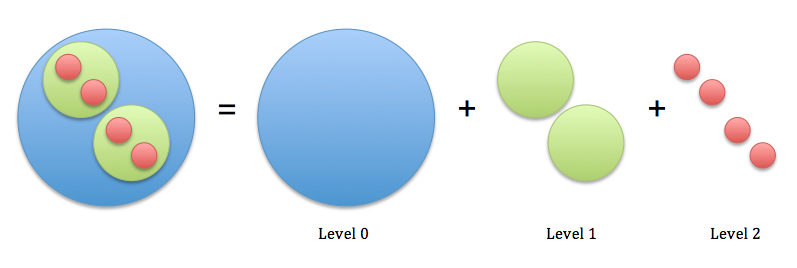
\includegraphics[width=0.7\textwidth]{multiresolution}
\end{figure}
\subsection{Datasets}
sdfsdf \\
sdfsd\\
sdfsd\\
sdfsdf\\
asdads\\
addfs\\
dsff\\


\newpage
\bibliographystyle{plain}
\bibliography{refs}

\end{document}